\begin{frame}{Frame Title}
\begin{figure}
    \centering
    \begin{subfigure}[b]{0.45\textwidth}
        \centering
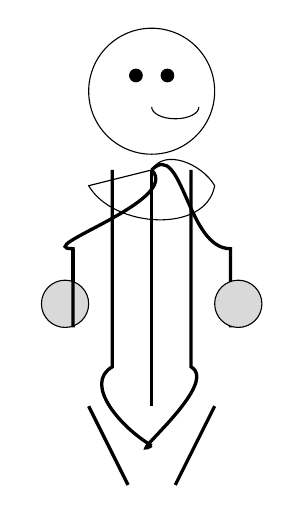
\begin{tikzpicture}
  % Head
  \draw (0,3) circle (0.8cm);
  \filldraw[black] (0.2,3.2) circle (0.08cm); % Eyes
  \filldraw[black] (-0.2,3.2) circle (0.08cm);
  \draw (0,2.8) arc (180:360: 0.3cm and 0.15cm); % Smirk

  % Body
  \draw[very thick] (0,2) to [out=45, in=180] (1,1) to (1,0); % Right arm
  \draw[very thick] (-1,1) -- (-1,0); % Right forearm
  \filldraw[fill=gray!30] (-1.1,0.3) circle (0.3cm); % Fist

  \draw[very thick] (0,2) to [out=-45, in=180] (-1,1) to (-1,0); % Left arm
  \draw[very thick] (1,1) -- (1,0); % Left forearm
  \filldraw[fill=gray!30] (1.1,0.3) circle (0.3cm); % Fist

  \draw[very thick] (0,2) -- (0,-1); 
  \draw[very thick] (0.8,-1) -- (0.3,-2); % Legs
  \draw[very thick] (-0.8,-1) -- (-0.3,-2); 
  % Legs (Improved)
  \draw[very thick] (0.5,2) -- (0.5,-0.5) to [out=-30,in=210] (0,-1.5); % Right leg
  \draw[very thick] (-0.5,2) -- (-0.5,-0.5) to [out=-150,in=150] (0,-1.5); % Left leg

  % Clothing
  \draw (0,2) to [out=60, in=120] (0.8, 1.8) to [out=260,in=300] (-0.8,1.8) --cycle; % Tanktop

 \end{tikzpicture}
\caption{GYMBro}
    \end{subfigure}
    \hfill
    \begin{subfigure}[b]{0.45\textwidth}
        \centering
        \begin{tikzpicture}[scale=0.5]
    % Head
    \fill[color=peach] (0,0) circle (1);
    % Hair
    \fill[color=black] (-1,0.8) -- (1,0.8) -- (1.5,1.8) -- (-1.5,1.8) -- cycle;
    % Face
    \fill[color=peach] (0,0) ellipse (0.8 and 0.5);
    % Eyes
    \fill[color=white] (-0.4,0.2) circle (0.1);
    \fill[color=white] (0.4,0.2) circle (0.1);
    \fill[color=black] (-0.4,0.2) circle (0.05);
    \fill[color=black] (0.4,0.2) circle (0.05);
    % Eyebrows
    \draw[color=black, line width=0.05cm] (-0.6,0.4) -- (-0.2,0.4);
    \draw[color=black, line width=0.05cm] (0.6,0.4) -- (0.2,0.4);
    % Mouth
    \draw[color=red, line width=0.05cm] (-0.2,-0.4) .. controls (0,-0.6) and (0, -0.6) .. (0.2,-0.4);
    % Body
    \fill[color=blue!30] (-1,-2) rectangle (1,-4.5);
    % Shoulders
    \fill[color=blue!30] (-2,-2) rectangle (-1,-1.7);
    \fill[color=blue!30] (2,-2) rectangle (1,-1.7);
    % Muscles
    \fill[color=blue!50] (-1.5,-1.7) rectangle (-0.5,-2.5);
    \fill[color=blue!50] (0.5,-1.7) rectangle (1.5,-2.5);
    % Arms
    \fill[color=blue!30] (-2.5,-2.5) rectangle (-1.5,-4);
    \fill[color=blue!30] (2.5,-2.5) rectangle (1.5,-4);
    % Dress
    \fill[color=blue!30] (-1.5,-4.5) rectangle (1.5,-6.5);
    % Legs
    \fill[color=pink] (-0.5,-6.5) rectangle (-1.5,-8);
    \fill[color=pink] (0.5,-6.5) rectangle (1.5,-8);
    % Shoes
    \fill[color=black] (-0.8,-8) rectangle (-1.2,-8.5);
    \fill[color=black] (0.8,-8) rectangle (1.2,-8.5);
    % Heels
    \fill[color=black] (-1,-8.5) rectangle (-1.4,-9);
    \fill[color=black] (1,-8.5) rectangle (1.4,-9);
\end{tikzpicture}
\caption{Human}
    \end{subfigure}
    \caption{Main caption}
    \label{fig:main}
\end{figure}

% \begin{tikzpicture}[scale=0.5]
%     % Head
%     \fill[color=peach] (0,0) circle (1);
%     % Hair
%     \fill[color=black] (-1,0.8) -- (1,0.8) -- (1.5,1.8) -- (-1.5,1.8) -- cycle;
%     % Face
%     \fill[color=peach] (0,0) ellipse (0.8 and 0.5);
%     % Eyes
%     \fill[color=white] (-0.4,0.2) circle (0.1);
%     \fill[color=white] (0.4,0.2) circle (0.1);
%     \fill[color=black] (-0.4,0.2) circle (0.05);
%     \fill[color=black] (0.4,0.2) circle (0.05);
%     % Eyebrows
%     \draw[color=black, line width=0.05cm] (-0.6,0.4) -- (-0.2,0.4);
%     \draw[color=black, line width=0.05cm] (0.6,0.4) -- (0.2,0.4);
%     % Mouth
%     \draw[color=red, line width=0.05cm] (-0.2,-0.4) .. controls (0,-0.6) and (0, -0.6) .. (0.2,-0.4);
%     % Body
%     \fill[color=pink] (-1,-2) rectangle (1,-4.5);
%     % Arms
%     \fill[color=pink] (-2.5,-2.5) rectangle (-1.5,-4);
%     \fill[color=pink] (2.5,-2.5) rectangle (1.5,-4);
%     % Dress
%     \fill[color=blue!30] (-1.5,-4.5) rectangle (1.5,-6.5);
%     % Legs
%     \fill[color=pink] (-0.5,-6.5) rectangle (-1.5,-8);
%     \fill[color=pink] (0.5,-6.5) rectangle (1.5,-8);
%     % Shoes
%     \fill[color=black] (-0.8,-8) rectangle (-1.2,-8.5);
%     \fill[color=black] (0.8,-8) rectangle (1.2,-8.5);
%     \end{tikzpicture}



%    \begin{tikzpicture}
%   % Head
%   \filldraw[fill=peach] (0,0) circle (1cm); % Skin tone

%   % Body (Hint of shoulders)
%   \draw [color=brown] (-1.2,-2) -- (0, -1.5) to [out=60, in=120] (1.2, -1.5) -- (1.2,-2);

%   % Eyes
%   \filldraw[fill=white] (0.4, 0.3) ellipse (0.25cm and 0.15cm); 
%   \filldraw[fill=brown] (0.4, 0.3) circle (0.07cm); % Iris
%   \filldraw[fill=white] (-0.4, 0.3) ellipse (0.25cm and 0.15cm); 
%   \filldraw[fill=brown] (-0.4, 0.3) circle (0.07cm); 

%   % Hair 
%   \filldraw[fill=black] (-1.2,0.3) to [out=-30,in=180] (0,1) to [out=0,in=150] (1.2,0.3);
%   \filldraw[fill=black] (-1.1,0) to [out=-20,in=180] (0,0.5) to [out=0,in=160] (1.1,0);

%   % Clothing (Example: Red dress)
%   \filldraw[fill=red, opacity=0.8] (-1.2,-2) -- (0, -1.5) to [out=60, in=120] (1.2, -1.5) -- (1,-3) -- (-1,-3)-- cycle; 
% \end{tikzpicture}


